%%%%%%%%%%%%%%%%%%%%%%%%%%%%%%%%%%%%%%%%%%%%%%%%%%%%%%%%%%%%%%%%%%%%%
% LaTeX Template: Project Titlepage Modified (v 0.1) by rcx
%
% Original Source: http://www.howtotex.com
% Date: February 2014
% 
% This is a title page template which be used for articles & reports.
% 
% This is the modified version of the original Latex template from
% aforementioned website.
% 
%%%%%%%%%%%%%%%%%%%%%%%%%%%%%%%%%%%%%%%%%%%%%%%%%%%%%%%%%%%%%%%%%%%%%%

\documentclass[12pt]{article}
\usepackage[a4paper]{geometry}
\usepackage[myheadings]{fullpage}
\usepackage{fancyhdr}

\usepackage{lastpage}
\usepackage{graphicx, wrapfig, subcaption, setspace, booktabs}
\usepackage[utf8]{inputenc}
\usepackage[T1]{fontenc}
%\usepackage[font=small, labelfont=bf]{caption}
\usepackage{fourier}
\usepackage[protrusion=true, expansion=true]{microtype}
\usepackage[french]{babel}
\usepackage{sectsty}
\usepackage{url, lipsum}


\newcommand{\HRule}[1]{\rule{\linewidth}{#1}}
\onehalfspacing
\setcounter{tocdepth}{5}
\setcounter{secnumdepth}{5}

%-------------------------------------------------------------------------------
% HEADER & FOOTER
%-------------------------------------------------------------------------------
\pagestyle{fancy}
\fancyhf{}
\setlength\headheight{15pt}
\fancyhead[L]{Emmanuel de Bézenac, Arthur Ramolet}
\fancyhead[R]{UPMC}
\fancyfoot[R]{\thepage\ / \pageref{LastPage}}
%-------------------------------------------------------------------------------
% TITLE PAGE
%-------------------------------------------------------------------------------

\begin{document}

\title{ \normalsize \textsc{COMPLEX}
		\\ [2.0cm]
		\HRule{0.5pt} \\
		\LARGE \textbf{\uppercase{Ordonnancement de tâches sur des machines en série}}
		\HRule{2pt} \\ [0.5cm]
		\normalsize \today \vspace*{5\baselineskip}}

\date{}

\author{
		Emmanuel de Bézenac, Arthur Ramolet \\ 
		Université Pierre et Marie Curie \\
		Année Universitaire 2015-2016 }

\maketitle

\newpage
\tableofcontents

\newpage
%-------------------------------------------------------------------------------
% Section title formatting
\sectionfont{\scshape}
%-------------------------------------------------------------------------------


%----------------------------------------------------------------------------------------
%	INTRO
%----------------------------------------------------------------------------------------
\clearpage
\newpage
\section{Introduction}

L'objet de ce projet est de trouver une bonne solution au problème de passage de pièces sur 3 machines dans un atelier de fabrication, de façon à minimiser la date fin d'ordonnancement des taches. Nous savons que ce problème est NP-Difficile, et donc que nombre de possibilitées à envisager est exponentiel en le nombre de taches. Nous devons donc trouver des méthodes qui puissent optimiser le temps de calcul associé au problème.

Nous chercherons d'abord de trouver un bonne solution au problème, tout en étant s'assurant de la qualité de notre solution: on utilisera donc un algorithme approché avec garantie de performance. Nous nous aiderons de l'algorithme de Johnson qui nous fournit une solution optimale (et en temps polynomial) au problème d'ordonnancement sur 2 machines. Nous tanterons ensuite de réduire la complexité de cet algorithme.


Puis, nous chercherons trouver une solution exacte à ce problème, en se basant sur une méthode  de 'Branch and Bound'. Nous chercherons ensuite des bornes inférieures et supérieures associés à cette méthode pour nous permettre d'explorer uniquement les branches intéressantes. Nous discuterons également de nos résultats suite à une implémentation de l'algorithme, de la complexité en temps temporelle ainsi qu'en espace mémoire en fonction de la taille des instances de problèmes données.

Nous finirons par discuter de méthodes envisageables pour optimiser nos algorithmes actuels, et tenterons de fournir une méthode au problème généralisé sur un nombre quelconque de machines. 

%----------------------------------------------------------------------------------------
%	PART 1
%----------------------------------------------------------------------------------------
\clearpage
\newpage
\section{Algorithme approché avec garantie de performance}


%------------------------------------------------

\subsection{3-Approché}

Pour montrer que l'ordonnancement associé à P, une permutation arbitraire est 3-approché, il suffit de montrer que : \\
\begin{center}
(1) $Cout(P) \le \displaystyle\sum_{i=1}^n(d_i^A+d_i^B+d_i^C)$\\
\end{center}
\begin{center}
(2) $OPT \ge \frac{1}{3}\displaystyle\sum_{i=1}^n(d_i^A+d_i^B+d_i^C)$\\
\end{center}
(1) et (2) nous donne bien :\\
\begin{center}
$3OPT \ge \displaystyle\sum_{i=1}^n(d_i^A+d_i^B+d_i^C) \ge Cout(P)$\\
\end{center}
L'ordonnancement associé à P serait donc 3-approché.\\

Montrons (1) : $Cout(P) \le \displaystyle\sum_{i=1}^n(d_i^A+d_i^B+d_i^C)$\\

$\displaystyle\sum_{i=1}^n(d_i^A+d_i^B+d_i^C)$ correspond à la date de fin d'ordonnancement des taches \{1,...,n\} lorsqu'on est obligé d'attendre que la tache i soit terminée sur la machine C, avant de pouvoir commencer la tache i+1 sur la machine A. Cela reviendrait à exécuter toutes les taches sur une seule machine (Au niveau de la date de fin, et en supposant qu'une machine puisse exécuter les taches des machines (A,B,C)). \\

En pratique, lorsque la tache i sur la machine A (respectivement B) est terminée on peut commencer directement la tache i+1 sur la machine B (respectivement C).\\

Remarque : Nous avons l'égalité lorsqu'il n'y a qu'une seule tache à effectuer.\\

Montrons maintenant (2) :\\

$\frac{1}{3}\displaystyle\sum_{i=1}^n(d_i^A+d_i^B+d_i^C)$ correspond à la durée moyenne de travail des machines A,B,C sur les taches \{1,...,n\}. Il y a forcément une machine qui prend d'avantage de temps à effectuer ses taches que la durée moyenne :\\
\begin{center}
(3) $\frac{1}{3}\displaystyle\sum_{i=1}^n(d_i^A+d_i^B+d_i^C) \le \max(\displaystyle\sum_{i=1}^n d_i^A,\displaystyle\sum_{i=1}^n d_i^B,\displaystyle\sum_{i=1}^n d_i^C)$\\
\end{center}
Comme toute les taches doivent passer sur chaque machine, nous avons :\\
\begin{center}
(4) $\max(\displaystyle\sum_{i=1}^n d_i^A,\displaystyle\sum_{i=1}^n d_i^B,\displaystyle\sum_{i=1}^n d_i^C) \le OPT$\\
\end{center}
avec (3) et (4) nous avons donc:\\
\begin{center}
$\frac{1}{3}\displaystyle\sum_{i=1}^n(d_i^A+d_i^B+d_i^C) \le OPT$\\

L'ordonnancement associé à P est donc 3-approché.
\end{center}
Exemples: Cas OPTIMAL et WSPT : \\ Soit $\epsilon$ > 0,et 3 taches \{1,2,3\} de durées :\\
\begin{center}
\begin{tabular}{|c|c|c|c|}
\hline 
Tache/Machine & A & B & C \\ 
\hline 
1 & $\epsilon$ & $\epsilon$ & 1 \\ 
\hline 
2 & $\epsilon$ & 1 & $\epsilon$ \\ 
\hline 
3 & 1 & $\epsilon$ & $\epsilon$ \\ 
\hline 
\end{tabular} 
\end{center}

\begin{figure}[!ht]
\centering
\centerline{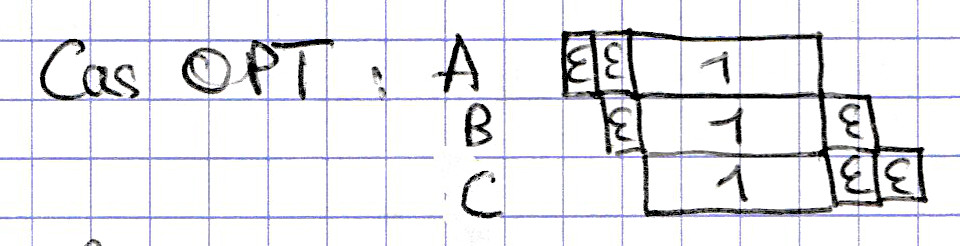
\includegraphics[scale=1]{1.jpg}}
\caption{Cas OPT}
\label{opt1}
\end{figure}

Lorsque $\epsilon$ -> 0, durée de fin = 1. avec permutation (1,2,3).

\begin{figure}[!ht]
\centering
\centerline{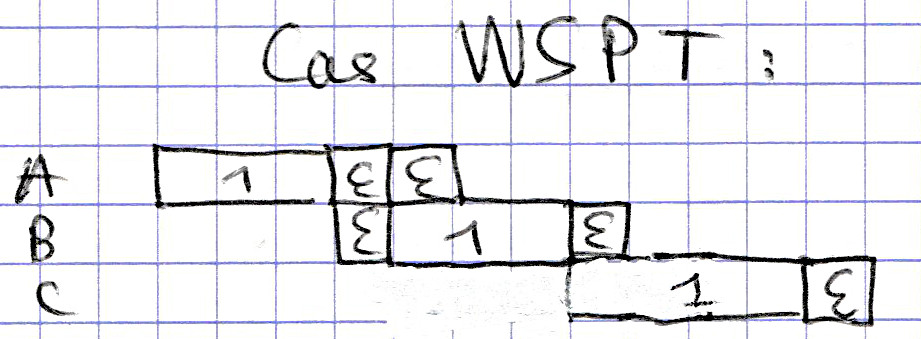
\includegraphics[scale=1]{2.jpg}}
\caption{Cas WSPT}
\label{wspt1}
\end{figure}

Lorsque $\epsilon$ -> 0, durée de fin = 3. avec permutation (3,2,1).

\subsection{2-Approché}

Soit $D_i^J$ la date de fin d'ordonnancement t retournée par l'algorithme de Johnson appliqué sur i machines.
L'inégalité suivante est triviale: Pour les deux problèmes (sur 2 et sur 3 machines) l'algorithme de Johnson nous renvoie la même permutation. Les Durées de fin d'ordonnancement sur les machines A et B sont donc identiques. Il reste à rajouter les taches de la machine C.   \\
\begin{center}
$D_3^J \le D_2^J + \displaystyle\sum_{i=1}^n d_i^C$\\
\end{center}
Nous avons bien l'énigalité, dans le second membre nous rajoutons les taches de C une fois que toutes les taches de B soient terminées.\\

Soient $OPT_3$ et $OPT_2$ étant la date de fin d'ordonnancement sur 3 machines (respectivement 2). Nous pouvons observer que (*) $D_2^J \le OPT_3$: la durée $D_2^J \ge OPT$ est optimale sur 2 machines, et on ne prend pas en compte les taches de la machine C.\\

Nous avons aussi (**)$\displaystyle\sum_{i=1}^n d_i^C \le OPT_3$: il y a au minimum la première tache de la machine A $D_i^A$ qui devrait être prise en compte).\\
\begin{center}
Avec (*) et (**) nous avons:
$D_3^J \le D_2^j + \displaystyle\sum_{i=1}^n d_i^C \le 2OPT$ 
\end{center}
Exemples: Cas OPTIMAL et WSPT : \\ Soit $\epsilon$ > 0,et 3 taches \{1,2,3\} de durées :\\
\begin{center}
\begin{tabular}{|c|c|c|c|}

\hline 
Tache/Machine & A & B & C \\ 
\hline 
1 & $\epsilon$ & 1 & $\epsilon$ \\ 
\hline 
2 & $\epsilon$ & $\epsilon$ & 1 \\ 
\hline 
3 & 1 & $\epsilon$ & $\epsilon$ \\ 
\hline 
\end{tabular} 
\end{center}
L'algorithme de Johnson nous renverrait la permutation (1,2,3), ce qui nous donne :

\begin{figure}[!ht]
\centering
\centerline{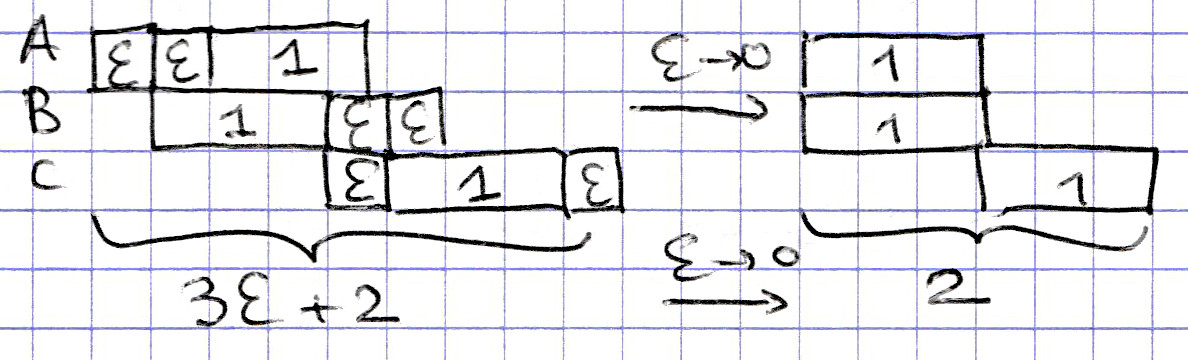
\includegraphics[scale=1]{3.jpg}}
\caption{Cas WSPT: Permutation selon l'algorithme de Johnson.}
\label{wspt2}
\end{figure}

\begin{figure}[!ht]
\centering
\centerline{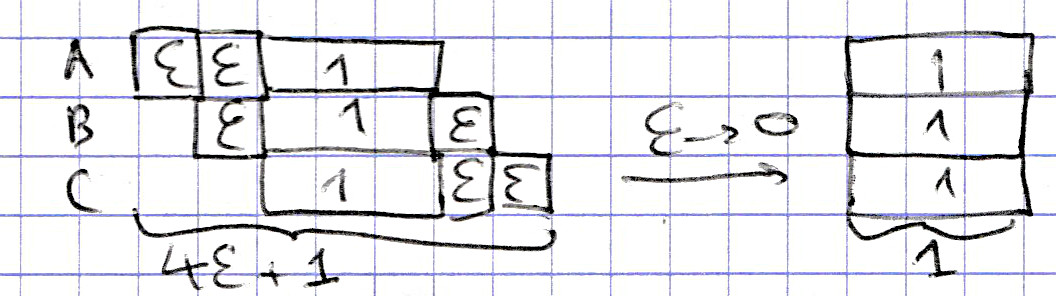
\includegraphics[scale=1]{4.jpg}}
\caption{Cas OPTIMAL, avec la permutation (2,1,3)}
\label{opt2}
\end{figure}


\subsection{Implémentation}

Nous avons choisi d'implémenter nos algorithmes avec langage C. La gestion "A la main" de la mémoire en permet une utilisation optimale, de plus le langage étant proche de la machine et notre compilateur (GCC) permettant l'optimisation du code via des flags (On utilisera -02 pour notre projet) nous garantie des performances accrues par rapport à un langage plus haut niveau. \\

Le développement sous GNU/Linux nous permet également d'utiliser facilement le timestamp UNIX afin de chronométrer nos temps d'exécutions avec une précision raisonnable (En théorie, en microsecondes. En pratique, pour de petites instances le temps est difficile a évaluer à cause des nombreuses opérations des différents algorithmes, donc plutôt de l'ordre de la dixième de microseconde (À la louche)).\\

Nous avons implémenté deux versions de l'algorithme de Johnson afin de comparer leurs performances. La première version est celle fournie dans le sujet. La seconde trie au préalable les taches dans l'ordre croissant afin pouvoir directement sélectionner les taches souhaitées. La complexité de la première version est en O($n^2$) alors que la seconde nous offre une complexité de O(n Log n). On confronte alors ces deux algorithmes pour des instances avec un nombre de taches variant de 1 à 2500. Les durées respectives sont générées aléatoirement selon 3 classes : Données non-corrélées, Corrélation sur les durées d'exécution et Corrélation sur les machines.\\

\begin{figure}[!ht]
\centering
\centerline{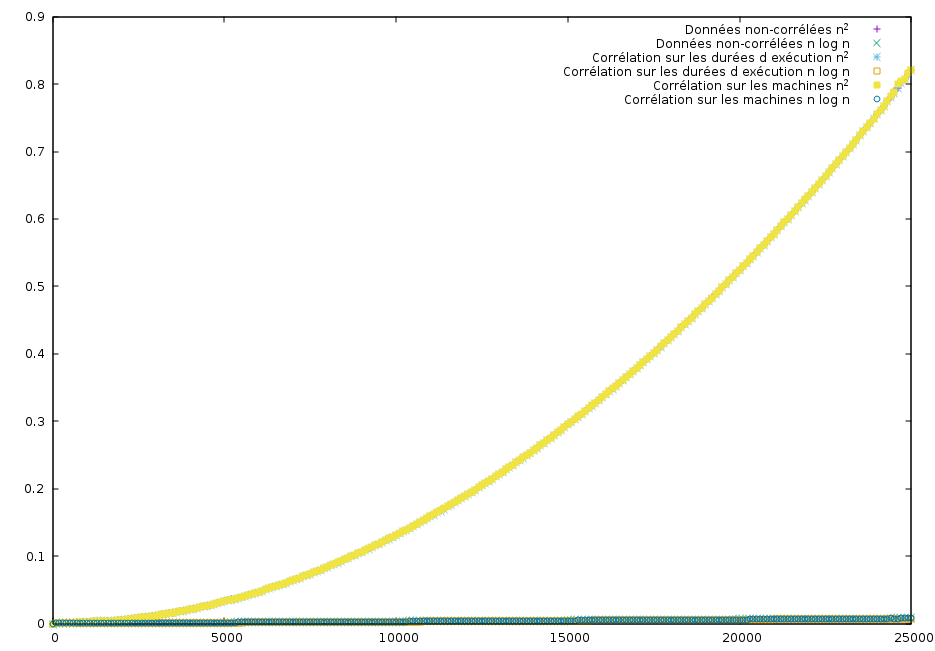
\includegraphics[scale=0.7]{johnson.png}}
\caption{Temps de calcul des algorithmes de johnson et des différentes classes de génération d'instance.}
\label{john}
\end{figure}

On observe (Fig : \ref{john}) que l'algorithme avec tri propose des performances nettement supérieures à l'algorithme original.
Celui-ci étant 2-approché, il pourra être utilisé afin de trouver une borne supérieure de notre instance.
On observe aussi que les différentes classes n'influent pas sur le déroulement de l'algorithme. (Les courbes sont confondues pour chaque classe).

%----------------------------------------------------------------------------------------
%	Part 2
%----------------------------------------------------------------------------------------
\clearpage
\newpage
\section{Méthode exacte}

\subsection{Première borne}

Montrons que dans $b_B^\pi$, on peut remplacer $t_B^\pi$ par :
(formule 12), c'est à dire $t_B^\pi \ge {t^\prime}_B^\pi$ (On cherche la plus grande borne inférieure).

\begin{figure}[!ht]
\centering
\centerline{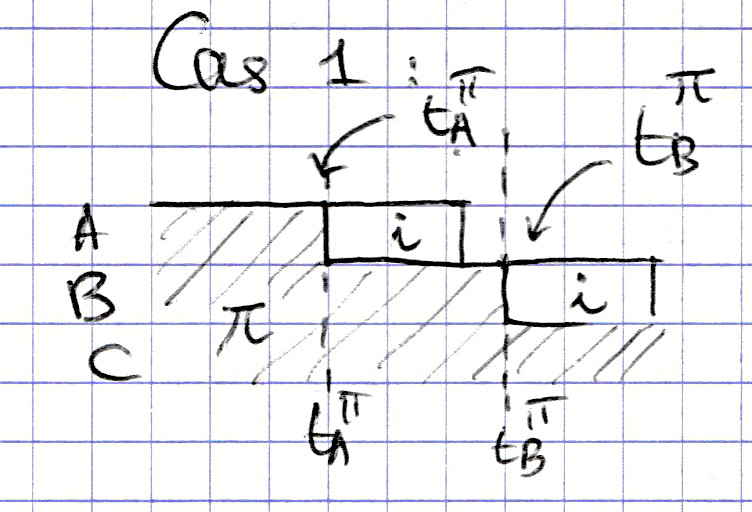
\includegraphics[scale=1]{5.jpg}}
\caption{Cas 1}
\label{cas11}
\end{figure}

Ici (Fig : \ref{cas11}), une fois les taches $\pi$ terminées sur A, on rajoute la tache i, $i\in{\pi}^\prime,i = {\arg\min\limits_{i\in{\pi^\prime}}}\{d_A^i\}$, pour ne pas perdre de généralité.

Ici, $t_A + d_A^i < t_B$. Il faudra alors attendre que les taches de $\pi$ se terminent sur B avant de pouvoir commencer la tache i sur B.

\begin{figure}[!ht]
\centering
\centerline{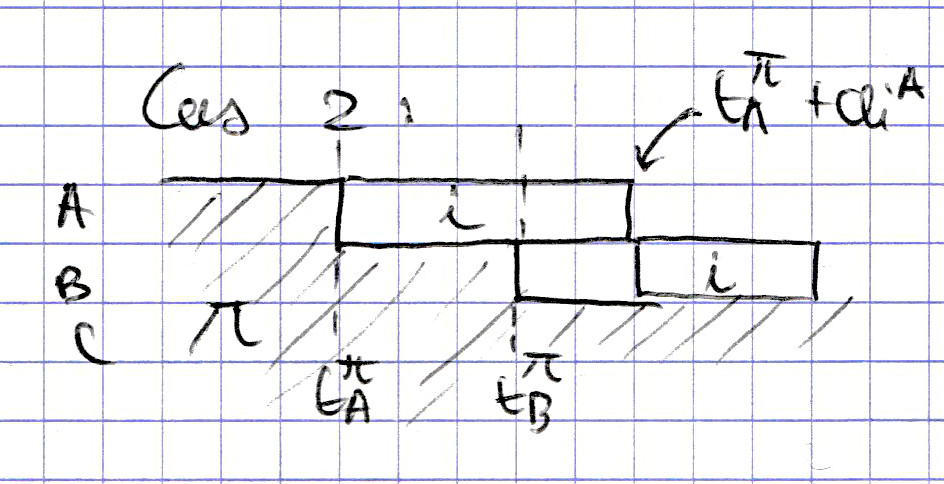
\includegraphics[scale=1]{6.jpg}}
\caption{Cas 2}
\label{cas12}
\end{figure}

Ici (Fig : \ref{cas12}) ,  $t_A + d_i^A \ge t_B$. Il faudra donc attendre que la tache i se termine sur A avant de la commencer sur B.

Au lieu d'uniquement prendre en compte $t_b^\pi$ pour la borne inférieur, ce serait plus efficace de prendre en compte au moins une durée en plus (ici $\min\limits_{i\in{\pi^\prime}}\{d_A^i\}$, car elle pourrait nous donner une borne inférieure plus grande (Cf cas 2).

On remplace donc $t_B^\pi$ par $\max\{t_B^\pi,\min\limits_{i\in{\pi^\prime}}\{d_A^i\}+t_A^\pi\}$.


Montrons maintenant, qu'on peut toujours obtenir une borne inférieure en remplaçant $t_C^\pi$ par ${t^\prime}_C^\pi$ :

On va faire un raisonnement analogue à (la première borne) qui consiste à chercher les taches contraignantes. On va également choisir les taches de durée minimale, pour ne pas perdre de généralité (Pour toute permutation de $\pi^\prime$, on aura toujours au moins le minimum).

\begin{figure}[!ht]
\centering
\centerline{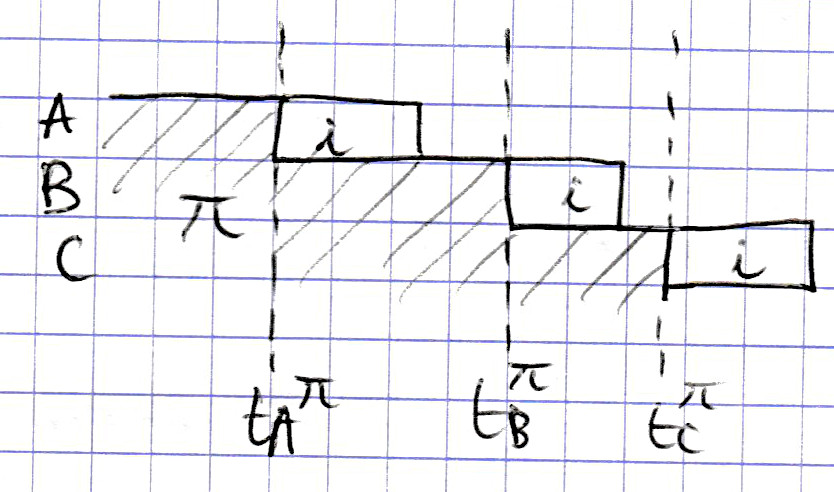
\includegraphics[scale=1]{7.jpg}}
\caption{Taches de $\pi$ contraignantes}
\label{cas21}
\end{figure}

Ici (Fig : \ref{cas21}) $t_C^\pi > t_B^\pi + \displaystyle\min_{i \in \pi^\prime}\{d_B^i\}$ et $t_C^\pi > t_A^\pi + \displaystyle\min_{i \in \pi^\prime}\{d_A^i + d_B^i\}$

\begin{figure}[!ht]
\centering
\centerline{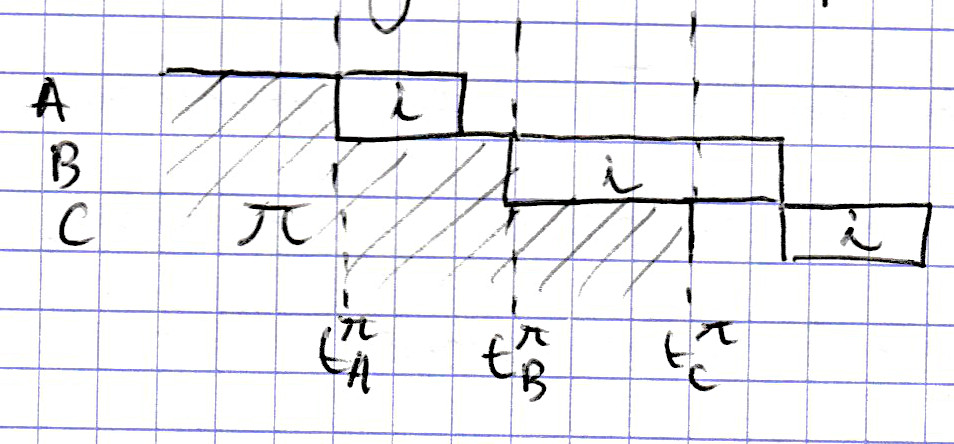
\includegraphics[scale=1]{8.jpg}}
\caption{Tache i sur machine B contraignante}
\label{cas22}
\end{figure}

Ici (Fig : \ref{cas22}) $t_B^\pi + \displaystyle\min_{i \in \pi^\prime}\{d_B^i\} > t_C^\pi$ et $t_B^\pi + \displaystyle\min_{i \in \pi^\prime}\{d_B^i\} > t_A^\pi + \displaystyle\min_{i \in \pi^\prime}\{d_A^i + d_B^i\}$


\begin{figure}[!ht]
\centering
\centerline{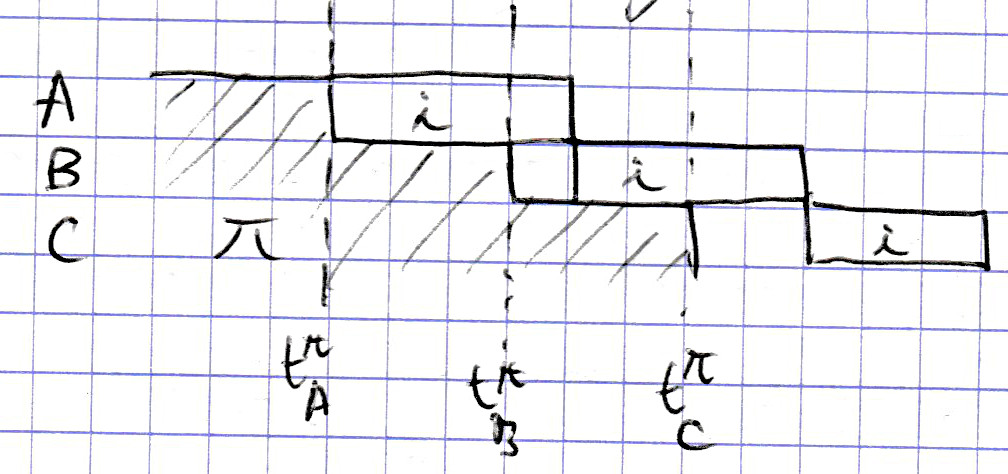
\includegraphics[scale=1]{9.jpg}}
\caption{Tache i sur machine A et B contraignante}
\label{cas23}
\end{figure}

Ici (Fig : \ref{cas23}) $t_A^\pi + \displaystyle\min_{i \in \pi^\prime}\{d_i^A + d_B^i\} > t_C$ et $t_A^\pi + \displaystyle\min_{i \in \pi^\prime}\{d_i^A + d_B^i\} > t_B + m...$ \\

Opter pour la borne inférieure de valeur maximale nous premet de construire une borne inférieure plus proche de la solution réalisable. Nous pourrons donc éspérer un élage plus fréquent des branches de l'arbre. En choisissant la tache minimale comme la première tache on ne perds pas de généralité car on est à la recherche d'une borne inférieure. (si la tache $i\in\pi^\prime$ était contraignante sur la machine $j\in\{A,B,C\}$, toutes les taches de $\pi^\prime$ le seraient également).

On peut donc remplacer $t_C^\pi$ par ${t^\prime}_C^\pi$, ce qui nous donne :\\
\begin{center}
${t^\prime}_C^\pi = \max\{t_C^\pi,t_B^\pi + \displaystyle\min_{i \in \pi^\prime} d_B^i, t_A^\pi + \displaystyle\min_{i \in \pi^\prime}\{d_A^i + d_B^i\}\}$
\end{center}

\subsection{Deuxième borne}

On schématise cette situation (Fig \ref{cas31}); pour simplifier, on suppose les taches \{1,...,k-1,k,k+1,...,n\} tel que : $d_i^A \le d_i^C, \forall i \in \{1,...,k-1\}$ et $d_i^A > d_i^C, \forall i \in \{k+1,...,n\}$

\begin{figure}[!ht]
\centering
\centerline{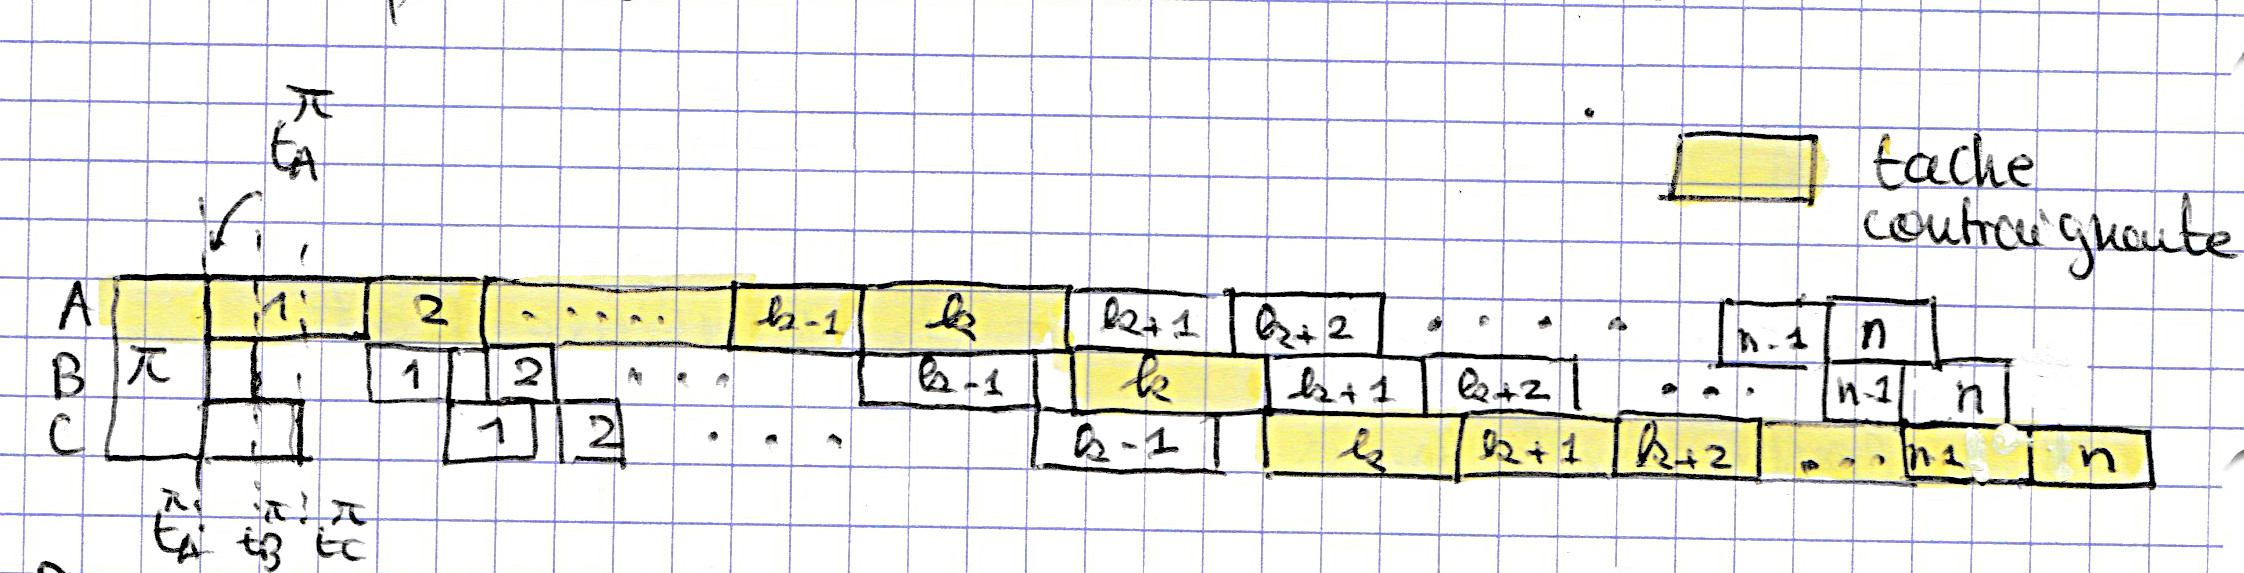
\includegraphics[scale=1]{10.jpg}}
\caption{}
\label{cas31}
\end{figure}

Pour simplifier, on suppose que les taches $\pi$ des machines B et C ne sont pas contraignantes (si elles l'était, on aurait un temps total égal ou plus grand). Pour que l'ordonnancement soit tel que sa date de fin soit corresponde à :\\
\begin{center}
$t_A^\pi + \displaystyle\sum_{d_A^i \le d_C^i}d_A^i + d_A^k + d_B^k + d_C^k + \displaystyle\sum_{d_A^i > d_C^i}d_C^i$\\
\end{center}
, il faudrait faire les suppositions fortes que les taches \{1,...,k\} soient contraignantes sur la machine A (Alors que par définition, on a $d_A^i \le d_C^i$), c'est à dire que ces mêmes taches ne soient pas contraignantes pour les machines B et C. Il faudrait également que les taches \{k+1,...,n\} soient contraignantes sur la machine C (alors que $d_i^A > d_i^C, \forall i \in \{k+1,...,n\}$.

On a que $\forall k \in \pi^\prime$ la date de fin d'ordonnancement associé à P est supérieure ou égale à cette borne inférieure. Pour trouver une borne inférieure, nous avons la liberté de choisir notre k, la meilleur option serait donc de choisir un k qui maximise notre borne, c'est à dire :\\
\begin{center}
 $b2 = t_A^\pi + \displaystyle\max_{k \in \pi^\prime}\{d_A^k + d_B^k + d_C^k + \displaystyle\sum_{i \in \pi^\prime,d_A^i \le d_C^i} d_A^i + \displaystyle\sum_{i \in \pi^\prime,d_A^i > d_C^i} d_C^i\} $\\
\end{center}
\subsection{Troisième borne}

En faisant le même raisonnement (Fig : \ref{cas41}), on peut déduire la borne :\\


\begin{center}
 $b3 = t_B^\pi + \displaystyle\max_{k \in \pi^\prime}\{d_B^k + d_C^k + \displaystyle\sum_{i \in \pi^\prime,d_B^i \le d_C^i} d_B^i + \displaystyle\sum_{i \in \pi^\prime,d_B^i > d_C^i} d_C^i\} $\\
\end{center}

\begin{figure}[!ht]
\centering
\centerline{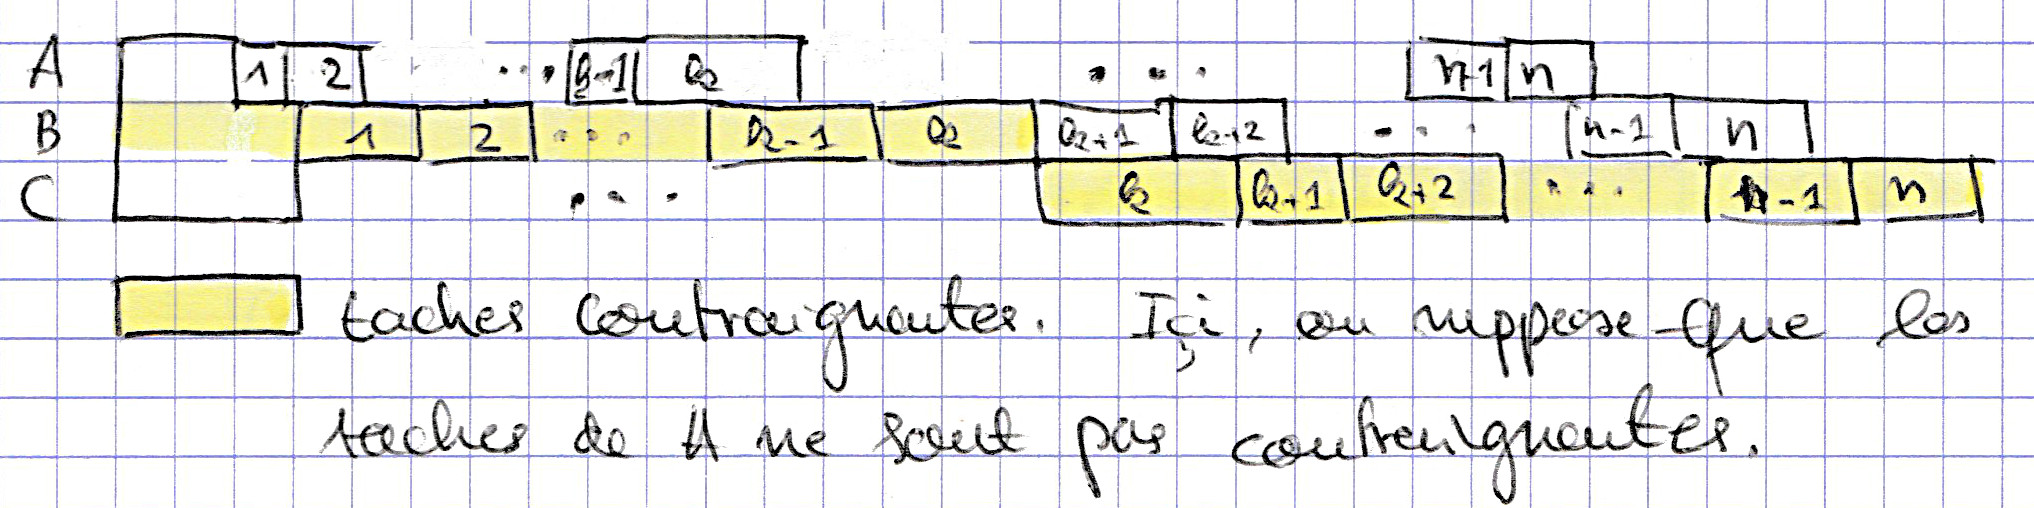
\includegraphics[scale=1]{11.jpg}}
\caption{}
\label{cas41}
\end{figure}

\subsection{Implémentation}

Pour traiter cette partie nous avons choisi le même langage pour les mêmes raisons que précédemment. Ainsi que pour une réutilisation aisée de l'algorithme de Johnson.\\

Ayant opté pour une implémentation récursive du branch and bound, celle-ci diffère un peu de celle vue en cours. Le cœur récursif de l'implémentation se charge d'effectuer toute les permutations possibles, et à chaque permutation, on calcule une borne supérieure et une borne inférieure. Celles-ci déterminent si oui ou non, l'exploration se poursuit dans la branche courante (comme traité en TD, pour un problème de minimisation). Nous avons choisi l'implémentation récursive car elle nous paraissait plus intuitive pour un parcours d'arbre et utilisant l'optimisation de GCC, la récursion est traitée comme une boucle avec une pile. En soit, après optimisation, le code doit fonctionner de la même façon que l'algorithme étudié en cours. 

L'algorithme pouvant difficilement traiter des instances à plus de 10 taches, ce sera notre taille maximale durant les tests. Les moyennes ont été calculées sur 200 tests.

\begin{figure}[!ht]
\centering
\centerline{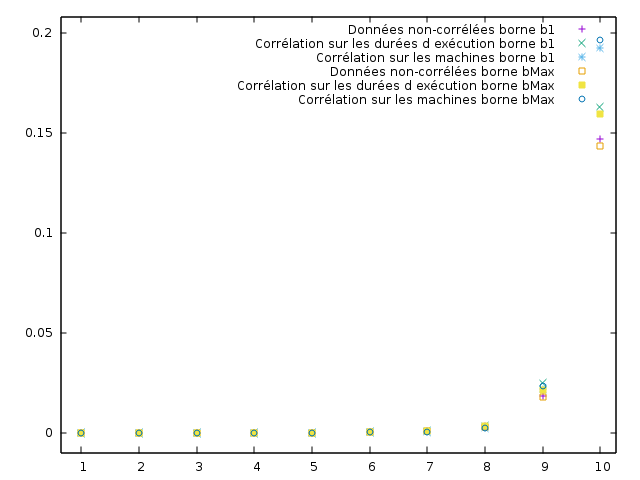
\includegraphics[scale=0.9]{tempsmoyen.png}}
\caption{Temps de calcul moyen pour pour les bornes b1 et bMax ainsi que des différentes classes de génération d'instance.}
\label{tmpmoy}
\end{figure}

\begin{figure}[!ht]
\centering
\centerline{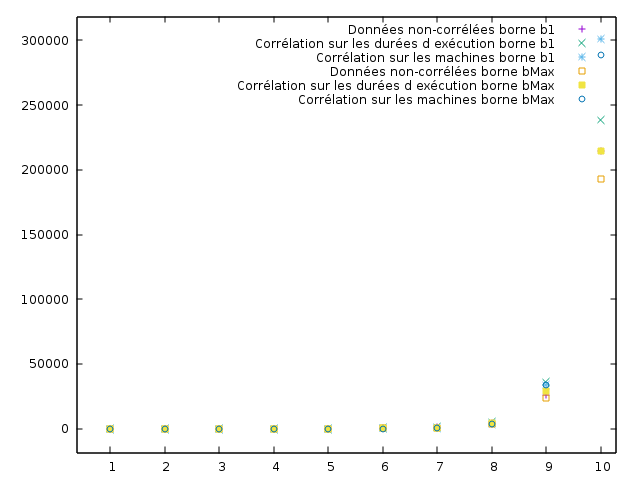
\includegraphics[scale=0.9]{nodemoyen.png}}
\caption{Nombre moyen de nœuds explorés pour les bornes b1 et bMax ainsi que des différentes classes de génération d'instance.}
\label{ndmoy}
\end{figure}

L'algorithme ne permettant pas le traitement de grandes instances, il est difficile de faire une analyse pertinente de nos résultats.

On constate que l'utilisation du branch and bound ne réduit pas la complexité dans le pire des cas (la complexité reste exponentielle), mais en pratique le temps de calcul est fortement diminué (Sur les figures \ref{tmpmoy} et \ref{ndmoy} mais explose avecle nombre de nœuds explorés à partir de 10 taches, et à 11 taches le temps de calcul est déjà trop élevé pour effectuer 200 tests avec chaque classe de génération).


On peut observer sur les temps d'exécutions (Fig : \ref{tmpmoy}) que :
La borne bMax dans les 3 classes montre des performances supérieures à la borne b1.
Les données non corrélées sont les plus rapides à être traitées, suivies des données corrélées sur les durées d'exécution et pour finir, les données corrélées. Il est possible d'observer un résultat similaire avec le nombre de nœuds explorés (Fig : \ref{ndmoy}).

On peut observer l'utilisation mémoire de l'algorithme pour une instance à 10 taches à l'aide de massif; un outil de valgrind.

\begin{figure}[!ht]
\centering
\centerline{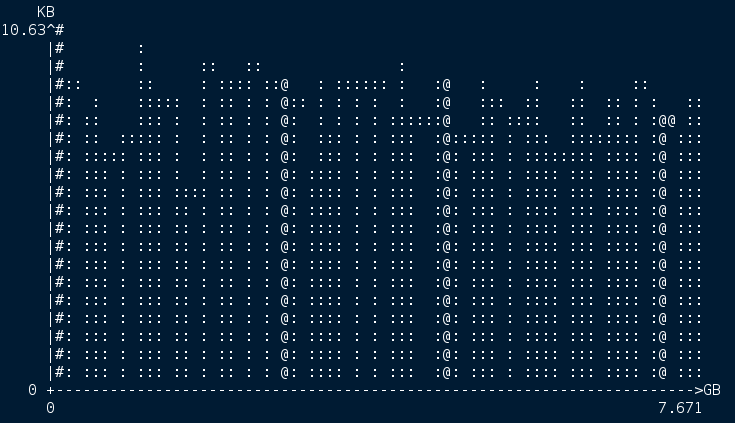
\includegraphics[scale=0.6]{mem.png}}
\caption{Occupation mémoire du branch and bound.}
\label{mem}
\end{figure}

On peut constater que l'allocation mémoire totale du programme est très lourde, c'est lié à l'implémentation de Johnson qui retourne une nouvelle instance à chaque appel. On pourrait réduire la consommation mémoire totale en modifiant cette implémentation. En contrepartie, l'allocation mémoire maximale durant le déroulement de l'algo est très faible (environ 11Ko). Cela permettrait traiter de grandes instances sans se soucier du problème de la mémoire.

%----------------------------------------------------------------------------------------

%----------------------------------------------------------------------------------------
%	PART 3
%----------------------------------------------------------------------------------------
\clearpage
\newpage
\section{Méthode de recherche arborescente approchée}

\subsection{Optimisations}

Il existe plusieurs méthodes qui pourraient encore réduire le temps de calcul moyen de manière significative.\\

Nous pouvons dans un premier temps modifier notre algorithme de Branch and Bound, pour effectuer un parcours en largeur modifié: l'algorithme explore toutes les branches en calculant pour chaque noeud une solution réalisable à l'aide de l'algorithme de Johnson. On emprunte en premier les branches les plus prometteuses, c'est-à-dire celles qui nous renvoie les meilleures solutions réalisables. En utilisant le même principe d'élagage des noeuds, nous pouvons aussi élaguer les branches dès que possible. Cette algorithme révisé nous permettrai potentiellement de trouver la meilleure solution dans un temps plus court (pour encore gagner du temps, nous pouvons nous très bien nous arrêter après un nombre quelconque k feuilles rencontrées, mais cette méthode ne serait plus exacte).

Nous pouvons ensuite aussi optimiser le temps de calcul en appliquant l'algorithme de Branch and Greed, c'est-à-dire choisir uniquement la branche qui nous rende la borne supérieure la plus faible, puis réitérer l'opération sur les branches du sous arbre. Cette méthode nous assure uniquement une solution convenable, mais nous assure une complexité de O($log(n)$) (nous descendons qu'une fois jusqu'à atteidre un noeud terminal). Cette méthode pourrait s'avérer utile pour de très grande instances. De plus, comme nous utilisons l'algorithme de Johnson, nous pouvons contrôler notre distance à l'ordonnancement optimal: notre solution serait au moins 2-approchée.

Faute de temps, nous étions dans l'incapacité d'implémenter ces méthodes.
%------------------------------------------------
\clearpage
\newpage
\section{Conclusion}


Nous avons pu constater qu'apporter des solutions à un problème NP-difficile est fastidieuse: l'algorithme approché avec garantie de performance nous renvoie des résultats convenables, mais il n'existe pas nécéssairement d'algorithmes approchés pour un problème NP-difficile (exemple: problème du voyageur de commerce). Il faut dans le cas échéant utiliser la méthode de branch and bound, qui nous assure une solution exacte, mais sans que la complexité dans le pire des cas soit réduite. Nous avons néenmoins des temps de calcul corrects pour des instances de taches qui restes petites, mais nous ne pourrons pas appliquer cette méthode pour des grandes instances. En optimisant cette méthode, il serait également possible d'avoir un temps de calcul en moyenne plus petit. Dans notre méthode exacte il est possible de baisser la complexité, sans pour autant trouver de solution en temps polynomial (sauf si P=NP). 
  
Nous nous sommes également aperçus que langage C n'est pas forcément pertinent dans le cadre de ce projet étudiant. En effet, même si les temps de calcul et l'occupation mémoire maximales sont intéressants, ces aspects sont peu intéressants dans cette étude. Les temps de calculs explosent trop rapidement pour rendre l'investissement consacré à la gestion de la mémoire et de l'optimisation intéressant par rapport à un langage plus haut niveau, qui nous aurais permis de traiter les parties manquantes.\\


%Figure : \ref{pouthisteqr}

%\newpage
%\begin{figure}[!t]
%\centering
%\centerline{\includegraphics{moon.jpg}}
%\caption{L'image moon.tif.}
%\label{moontif}
%\end{figure}



\end{document}
